\section{Assignment 3}

\subsection{Introduction}
In this assignment, we will study the behavior of a system of ordinary differential equations that models the dynamics of a cell, also known as `cell motility'. The system is given by
\begin{equation}
    \begin{cases}
        \hat{R}'_a &= \frac{\hat{A} \left(1 - \hat{R}_{a}\right)}{\hat{\rho}_a^{n} + \rho_{0}^{n}}  - \hat{\delta}_{R} \hat{R}_{a}\\
        \hat{\rho}'_a &= \frac{\hat{B} \left(1 - \hat{\rho}_a\right)}{\hat{R}_0^{n} + \hat{R}_{a}^{n}} - \hat{\rho}_a\\
    \end{cases}
\label{eq:cell_biology}
\end{equation}
As stated in the assignment, the goal here is to:
`\textit{to investigate the effect of changes in the parameter $\hat{B}$ due to external stimuli. Focus is on
comparing the model behavior under quasi-stationary and time-dependent parameter variations}'

\subsection{Autonomous system}
Figure \ref{fig:cell_biology_ex1} shows the continuation of the system with the following parameters (default): $R_0 = 0.3$, $\rho_0 = 0.16$, $\delta R = 1$, $n = 4$, $B_{max} = 0.04$ and $\epsilon = 0.0$. 

\begin{figure}[H]
    \centering
    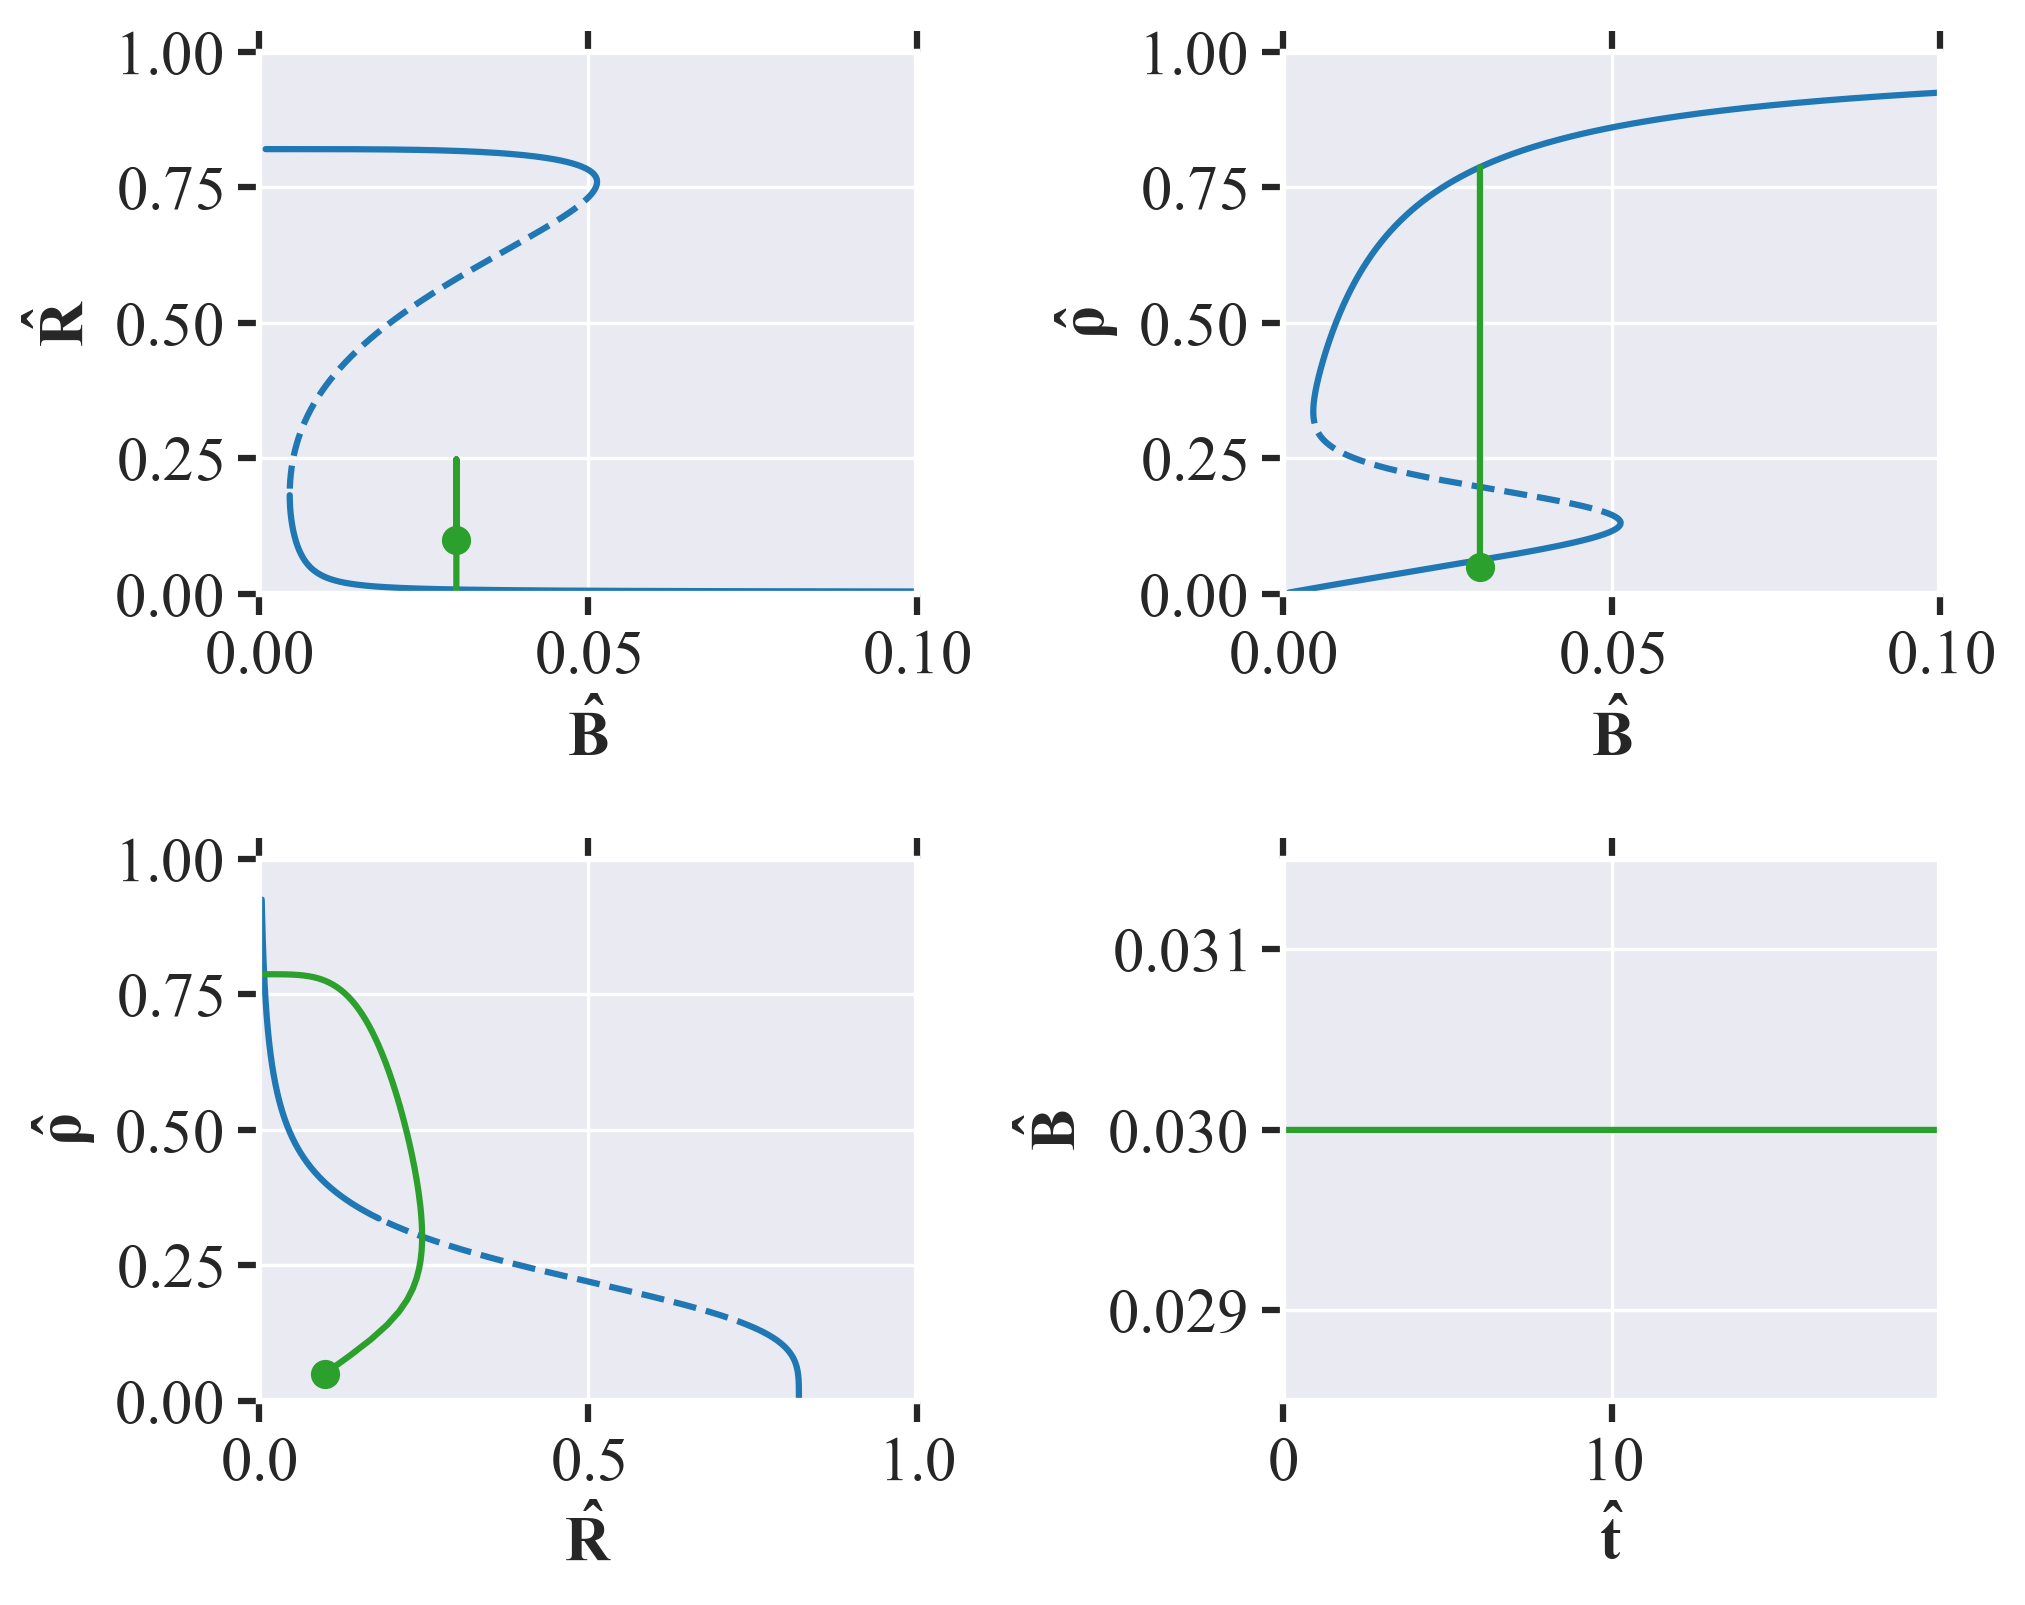
\includegraphics[width= \textwidth]{figures/cell_biology_R0=0.3_rho0=0.16_deltaR=1_n=4_Bmax=0.04_eps=0.0.png}
    \caption{Figure of the continuation of \textbf{top left:} $(\hat{R}, \hat{B})$ and \textbf{top right:}, $(\hat{\rho}, \hat{B})$, \textbf{bottom left:} phase space $(\hat{\rho}, \hat{R})$ and 
    \textbf{bottom right:} $\hat{B}$ against time (time horizon of 20 seconds with a time step of 0.01). Dots (orange) indicate turning points.}
    \label{fig:cell_biology_ex1}
\end{figure}

The system is at this stage effectively autonomous, since $\hat{B}(\hat{t}) \equiv \hat{B}_c$ is taken to be constant. Continuation is subsequently done with respect to the parameter $\hat{B}$. We observe two turning point bifurcations at:
\begin{enumerate}
    \item $\hat{B} \approx 0.051, \hat{R}\approx0.759, \hat{\rho}\approx0.131$; 
    \item $\hat{B} \approx 0.005, \hat{R}\approx0.182, \hat{\rho}\approx0.337$.
\end{enumerate}

Using the graph to get initial guesses for our Newton root finding method, we find there exist three equilibrium:
\begin{align*}
    E_0=(\hat{R_a}, \hat{\rho_a}) \approx (0.58,0.20) \leftarrow ||E_0|| \approx 0.61, \\
    E_1=(\hat{R_a}, \hat{\rho_a}) \approx (0.01,0.79) \leftarrow ||E_1|| \approx 0.79, \\
    E_2=(\hat{R_a}, \hat{\rho_a}) \approx (0.82,0.06) \leftarrow ||E_2|| \approx 0.82.
\end{align*}
$E_0$ is unstable, while $E_1$ and $E_2$ are stable. Moreover, looking at the trajectory in the phase space $(\hat{\rho}, \hat{R})$, we see that the system converges to $E_1$. 
Therefore, $E_1$ is the attractor in this case.

In figure \ref{fig:cell_biology_domains_of_attraction} the domains of attraction of $E_i, \ i = 1,2,3$ are shown.
\begin{figure}[H]
    \centering
    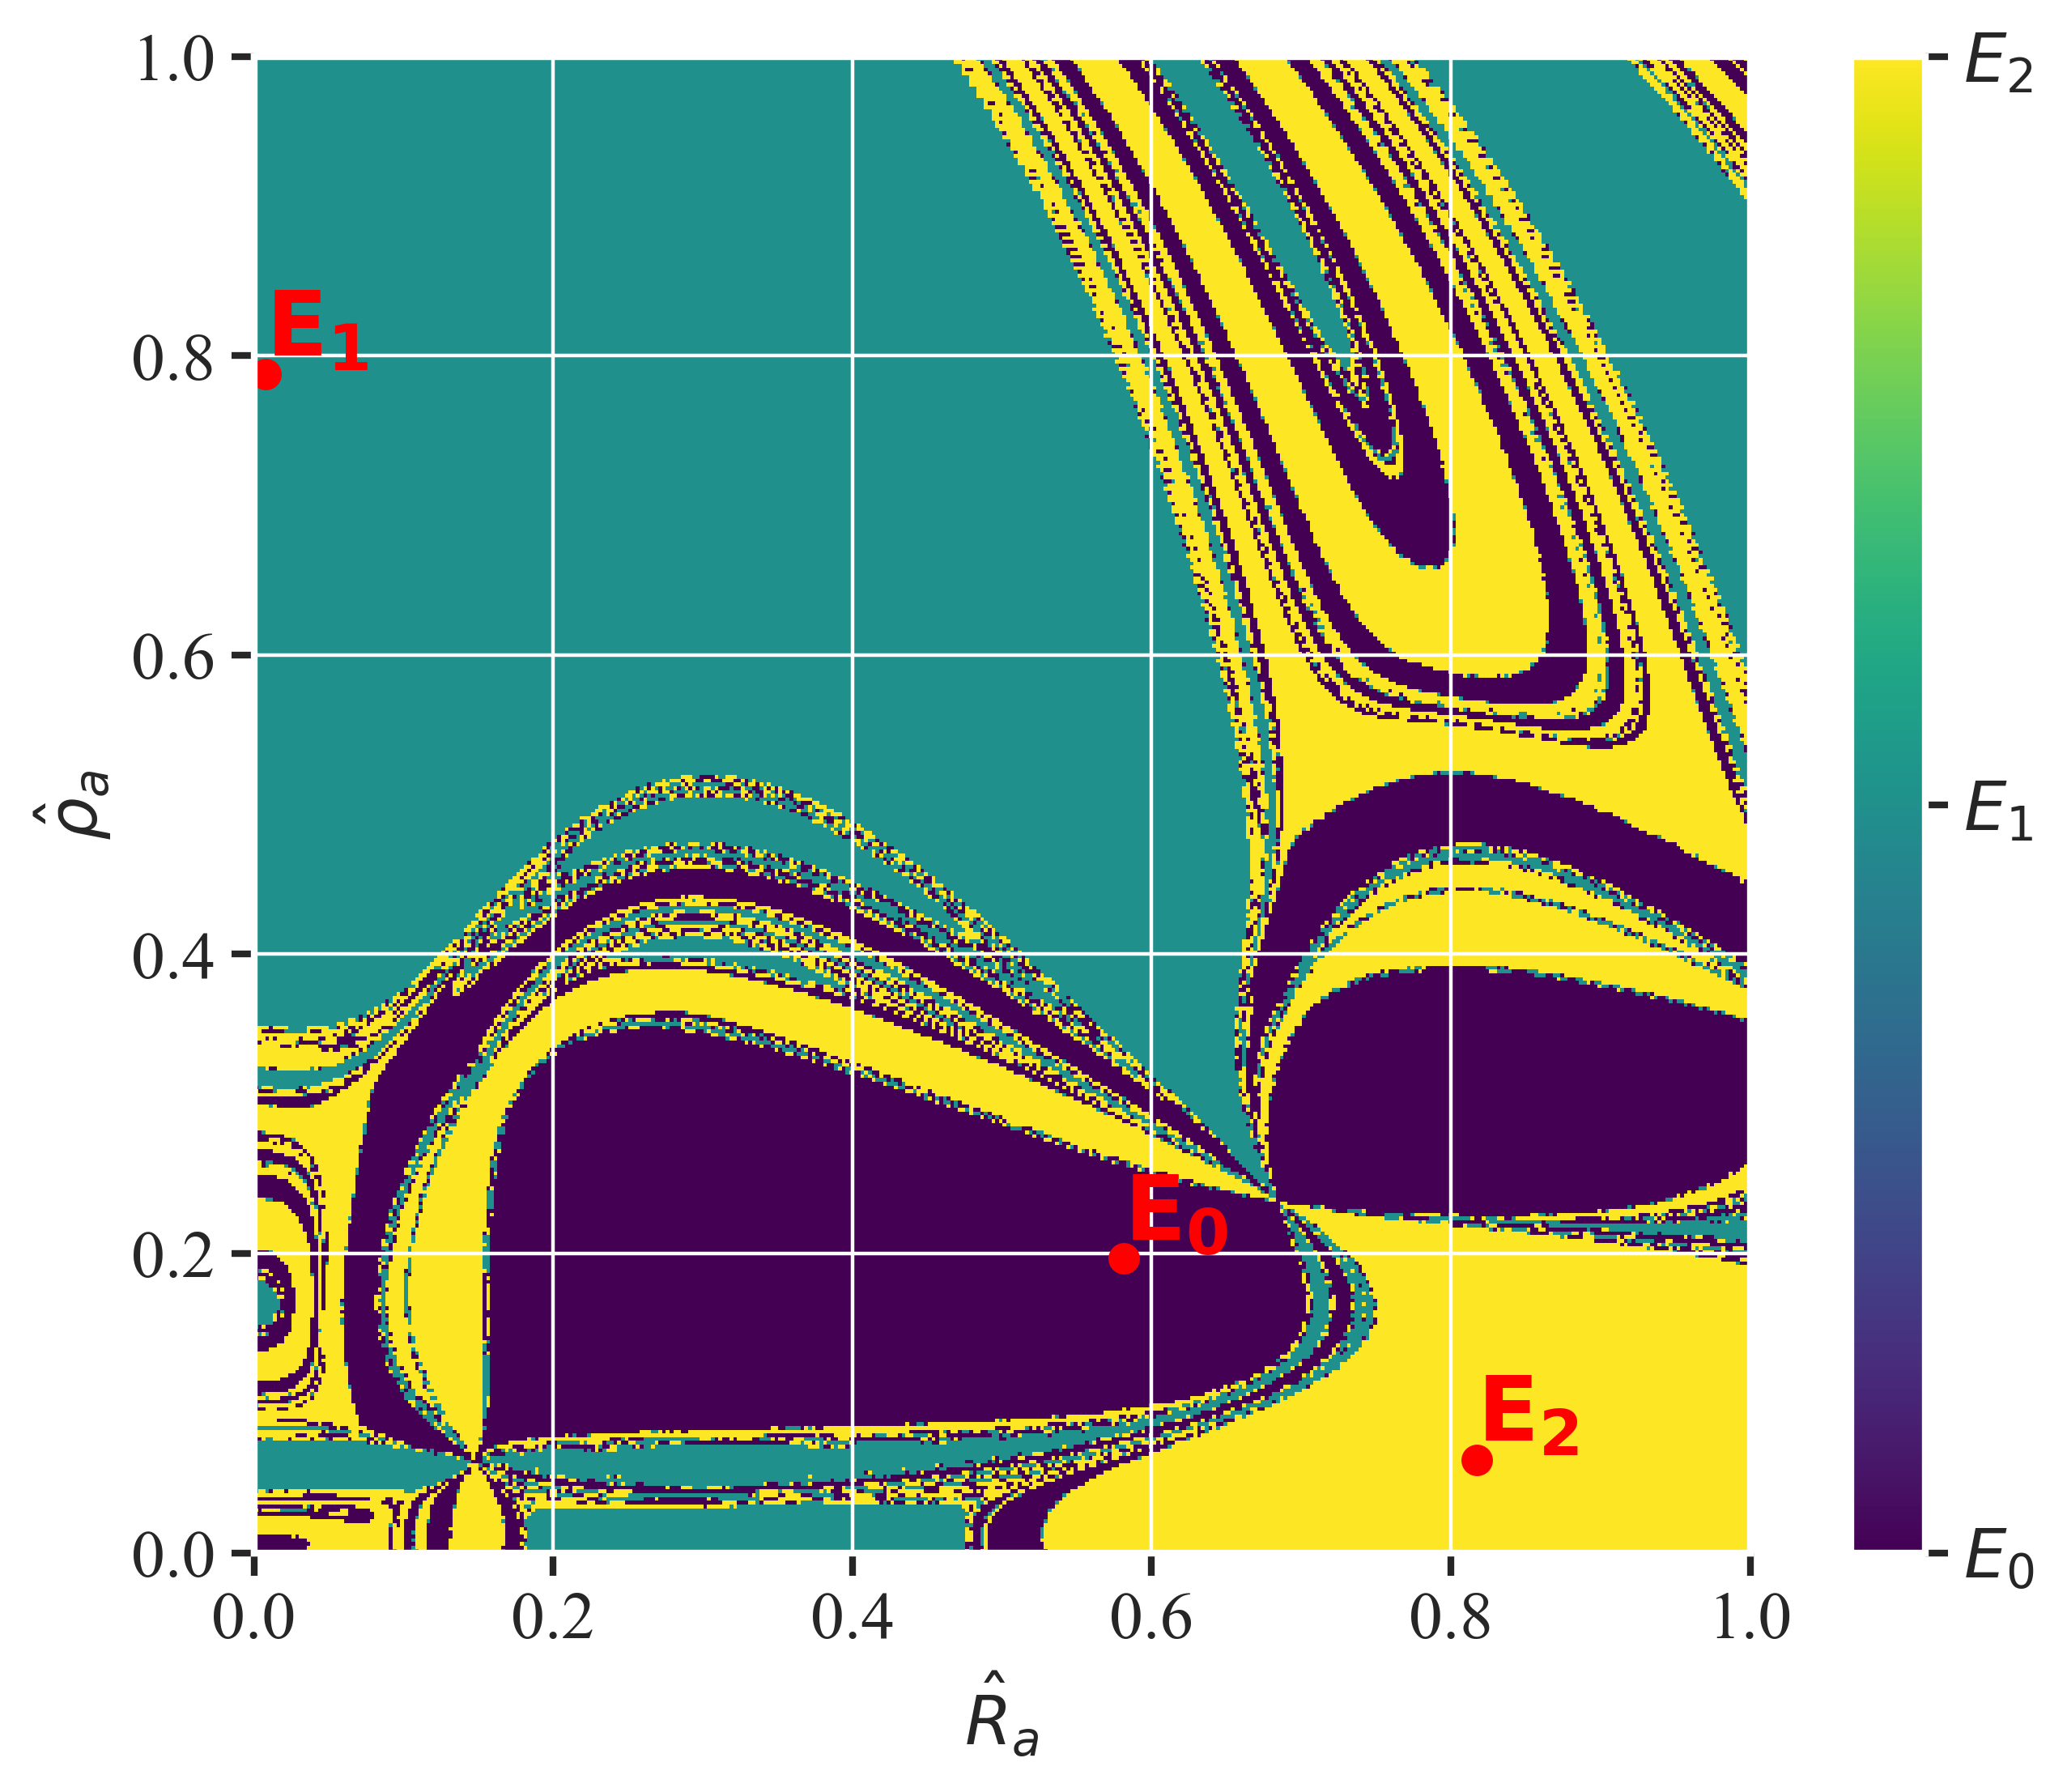
\includegraphics[width= \textwidth]{figures/cb_domains_of_attraction.png}
    \caption{Domains of attraction of $E_i, \ i = 1,2,3$. The color of a certain area in the plot indicates which equilibrium point the system converges to (purple to $E_0$, yellow to $E_1$ and cyan to $E_2$). 
    This is done by performing a Newton root finding method on a grid of initial conditions in the phase space $(\hat{\rho}, \hat{R})$. The red dots indicate the equilibrium points themselves. 
    Close to the equilibrium points, the system converges to the equilibrium point itself, in keeping with the theory on Newton(-like) methods. However, further away from the equilibrium 
    points, we get an amazingly complex mixture of the various domains of attractions. Looks like someone folded hyperspace in on itself and slapped it flat, so we could see it.}
    \label{fig:cell_biology_domains_of_attraction}
\end{figure}

\subsection{Non-autonomous system}
We now introduce a `small' linear time-dependent perturbation to $\hat{B}$. That is, the perturbed system is now given by
\begin{equation}
    \begin{cases}
        \hat{R}'_a &= \frac{\hat{A} \left(1 - \hat{R}_{a}\right)}{\hat{\rho}_a^{n} + \rho_{0}^{n}}  - \hat{\delta}_{R} \hat{R}_{a}\\
        \hat{\rho}'_a &= \frac{\hat{B} \left(1 - \hat{\rho}_a\right)}{\hat{R}_0^{n} + \hat{R}_{a}^{n}} - \hat{\rho}_a\\
        \hat{B}' &= \epsilon,
    \end{cases}
\label{eq:cell_biology_linear_perturbation}
\end{equation}
where $\epsilon$ is small or big with respect to the linearized system dynamics (reciprocal of the linearized system's eigenvalues). 

Figures \ref{fig:cell_biology_ex3_small} and \ref{fig:cell_biology_ex3_big} show the continuation of the autonomous system, as well as a trajectory of the 
system for $\epsilon = 0.0001$ and $\epsilon = 0.01$ respectively. 
For small $\epsilon$, the system has sufficient time to restore to its autonomous (quasi-)equilibrium. This is no longer the case for big $\epsilon$. 
\begin{figure}[H]
    \centering
    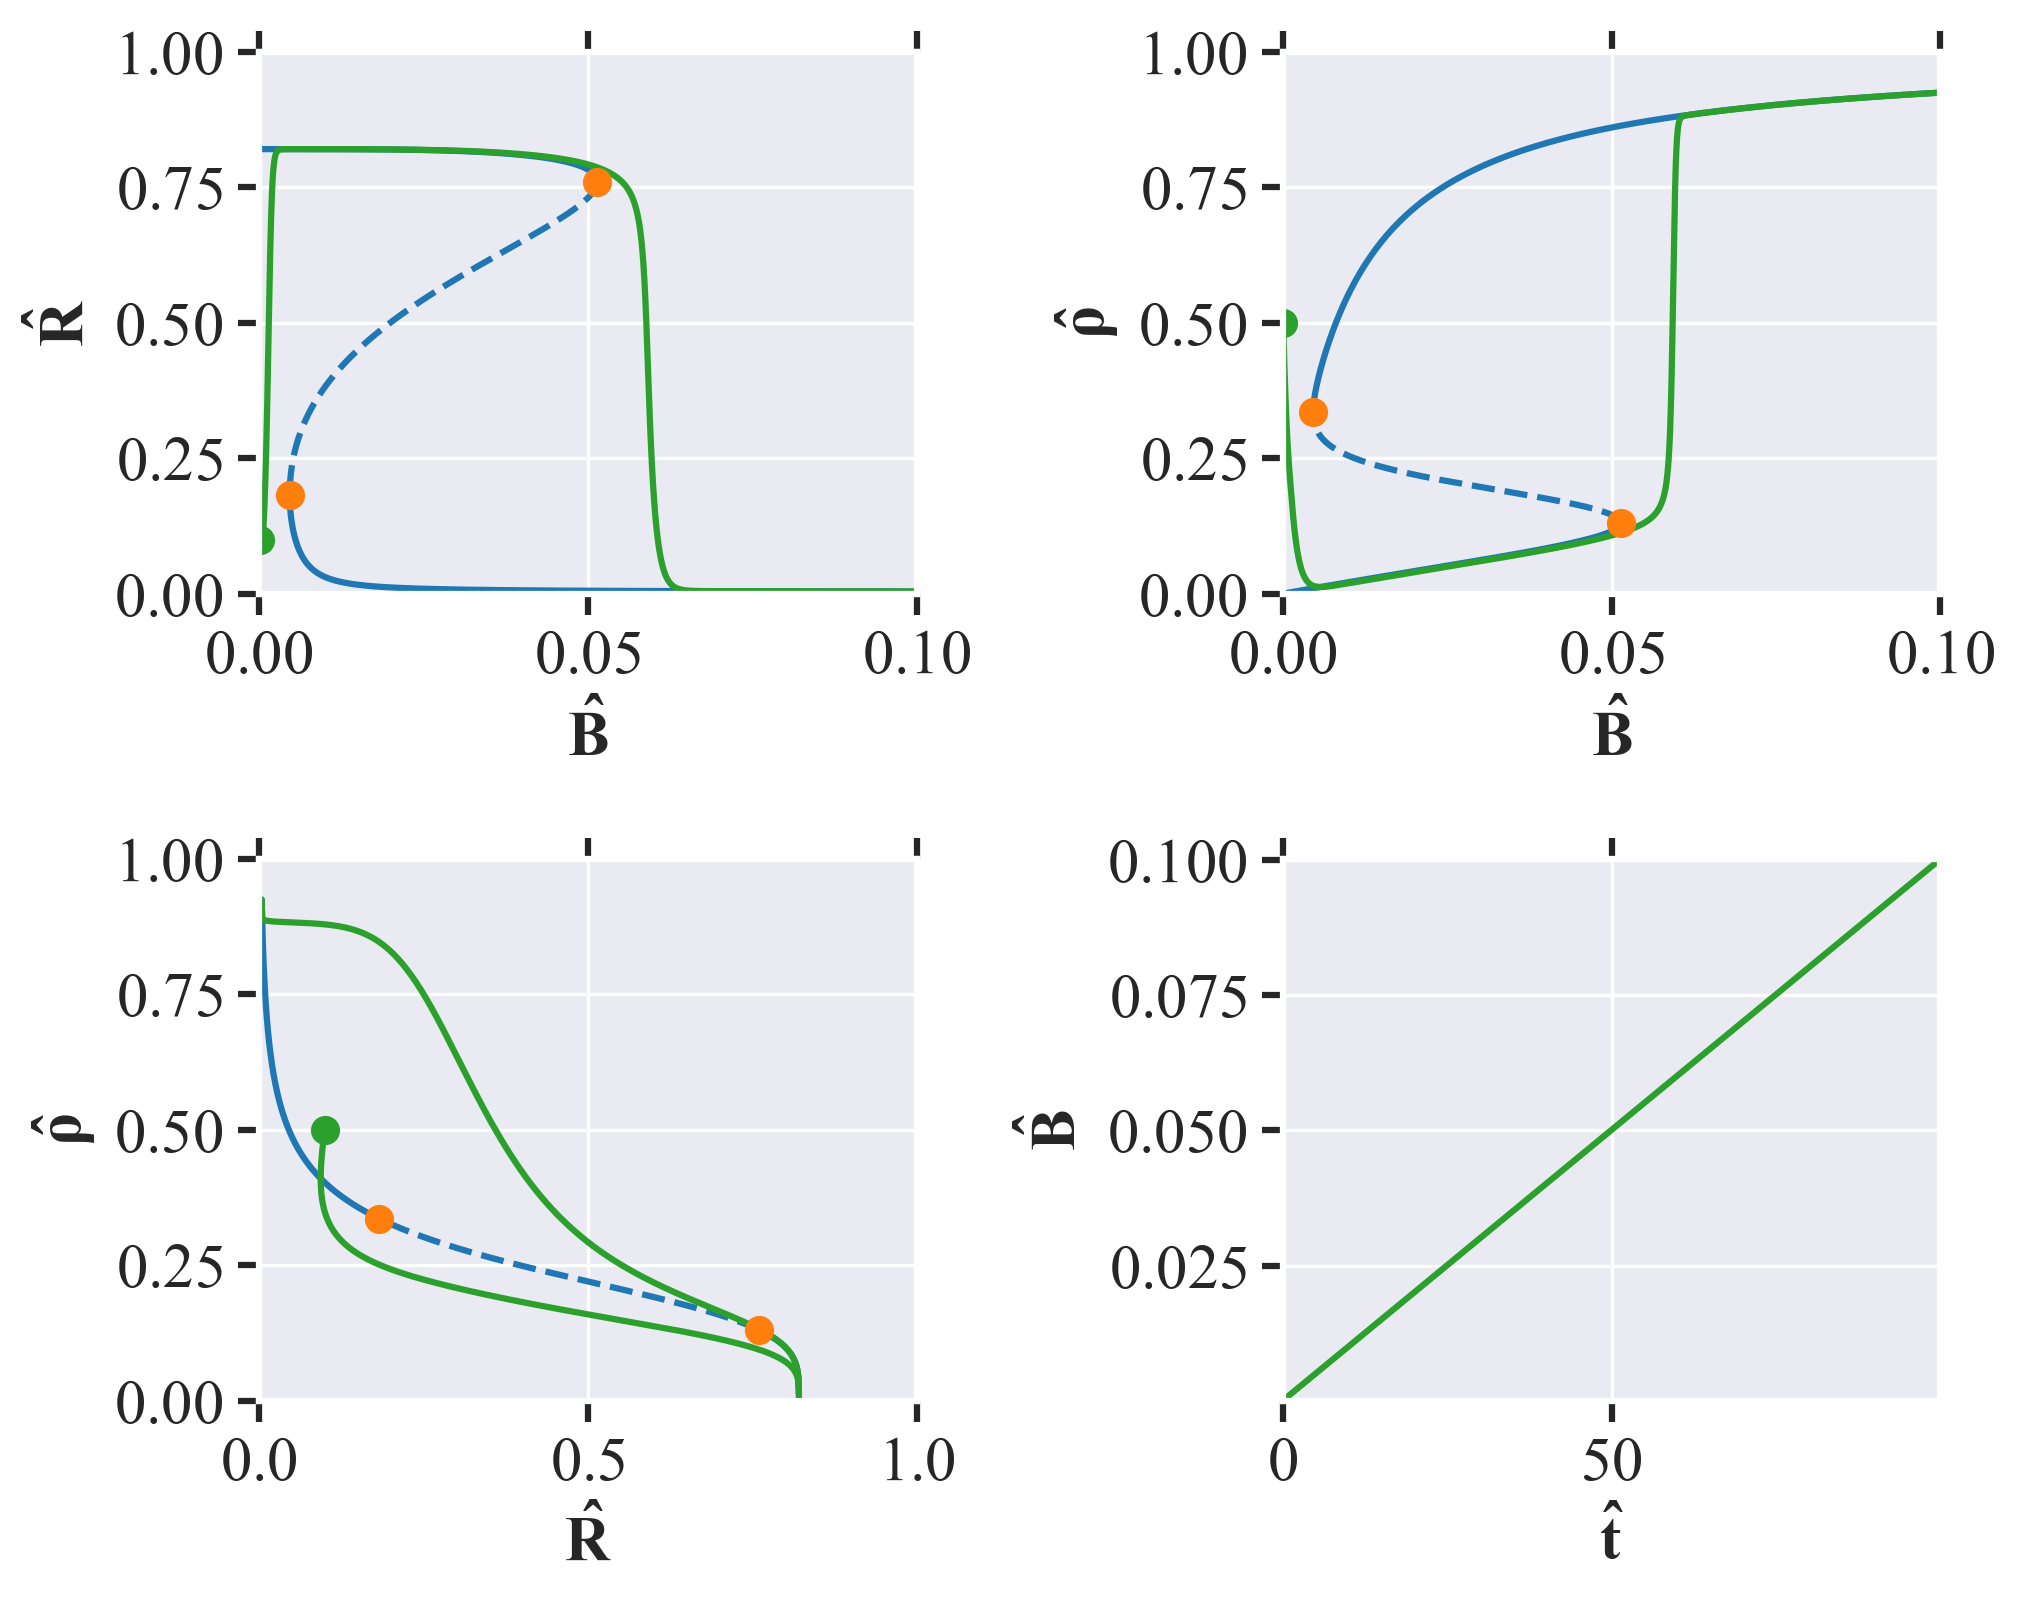
\includegraphics[width= \textwidth]{figures/cell_biology_R(0)=0.1_rho(0)=0.5_B(0)_0.0001_eps=0.001_Bmax=0.04.png}
    \caption{System behavior for small $\epsilon = 0.0001$. Plotted are the unperturbed system's equilibria and a trajectory of the perturbed system with initial condition
    $(\hat{R}_0, \hat{\rho}_0) = (0.1, 0.5)$ and time horizon $T = 100$.}
    \label{fig:cell_biology_ex3_small}
\end{figure}

\begin{figure}[H]
    \centering
    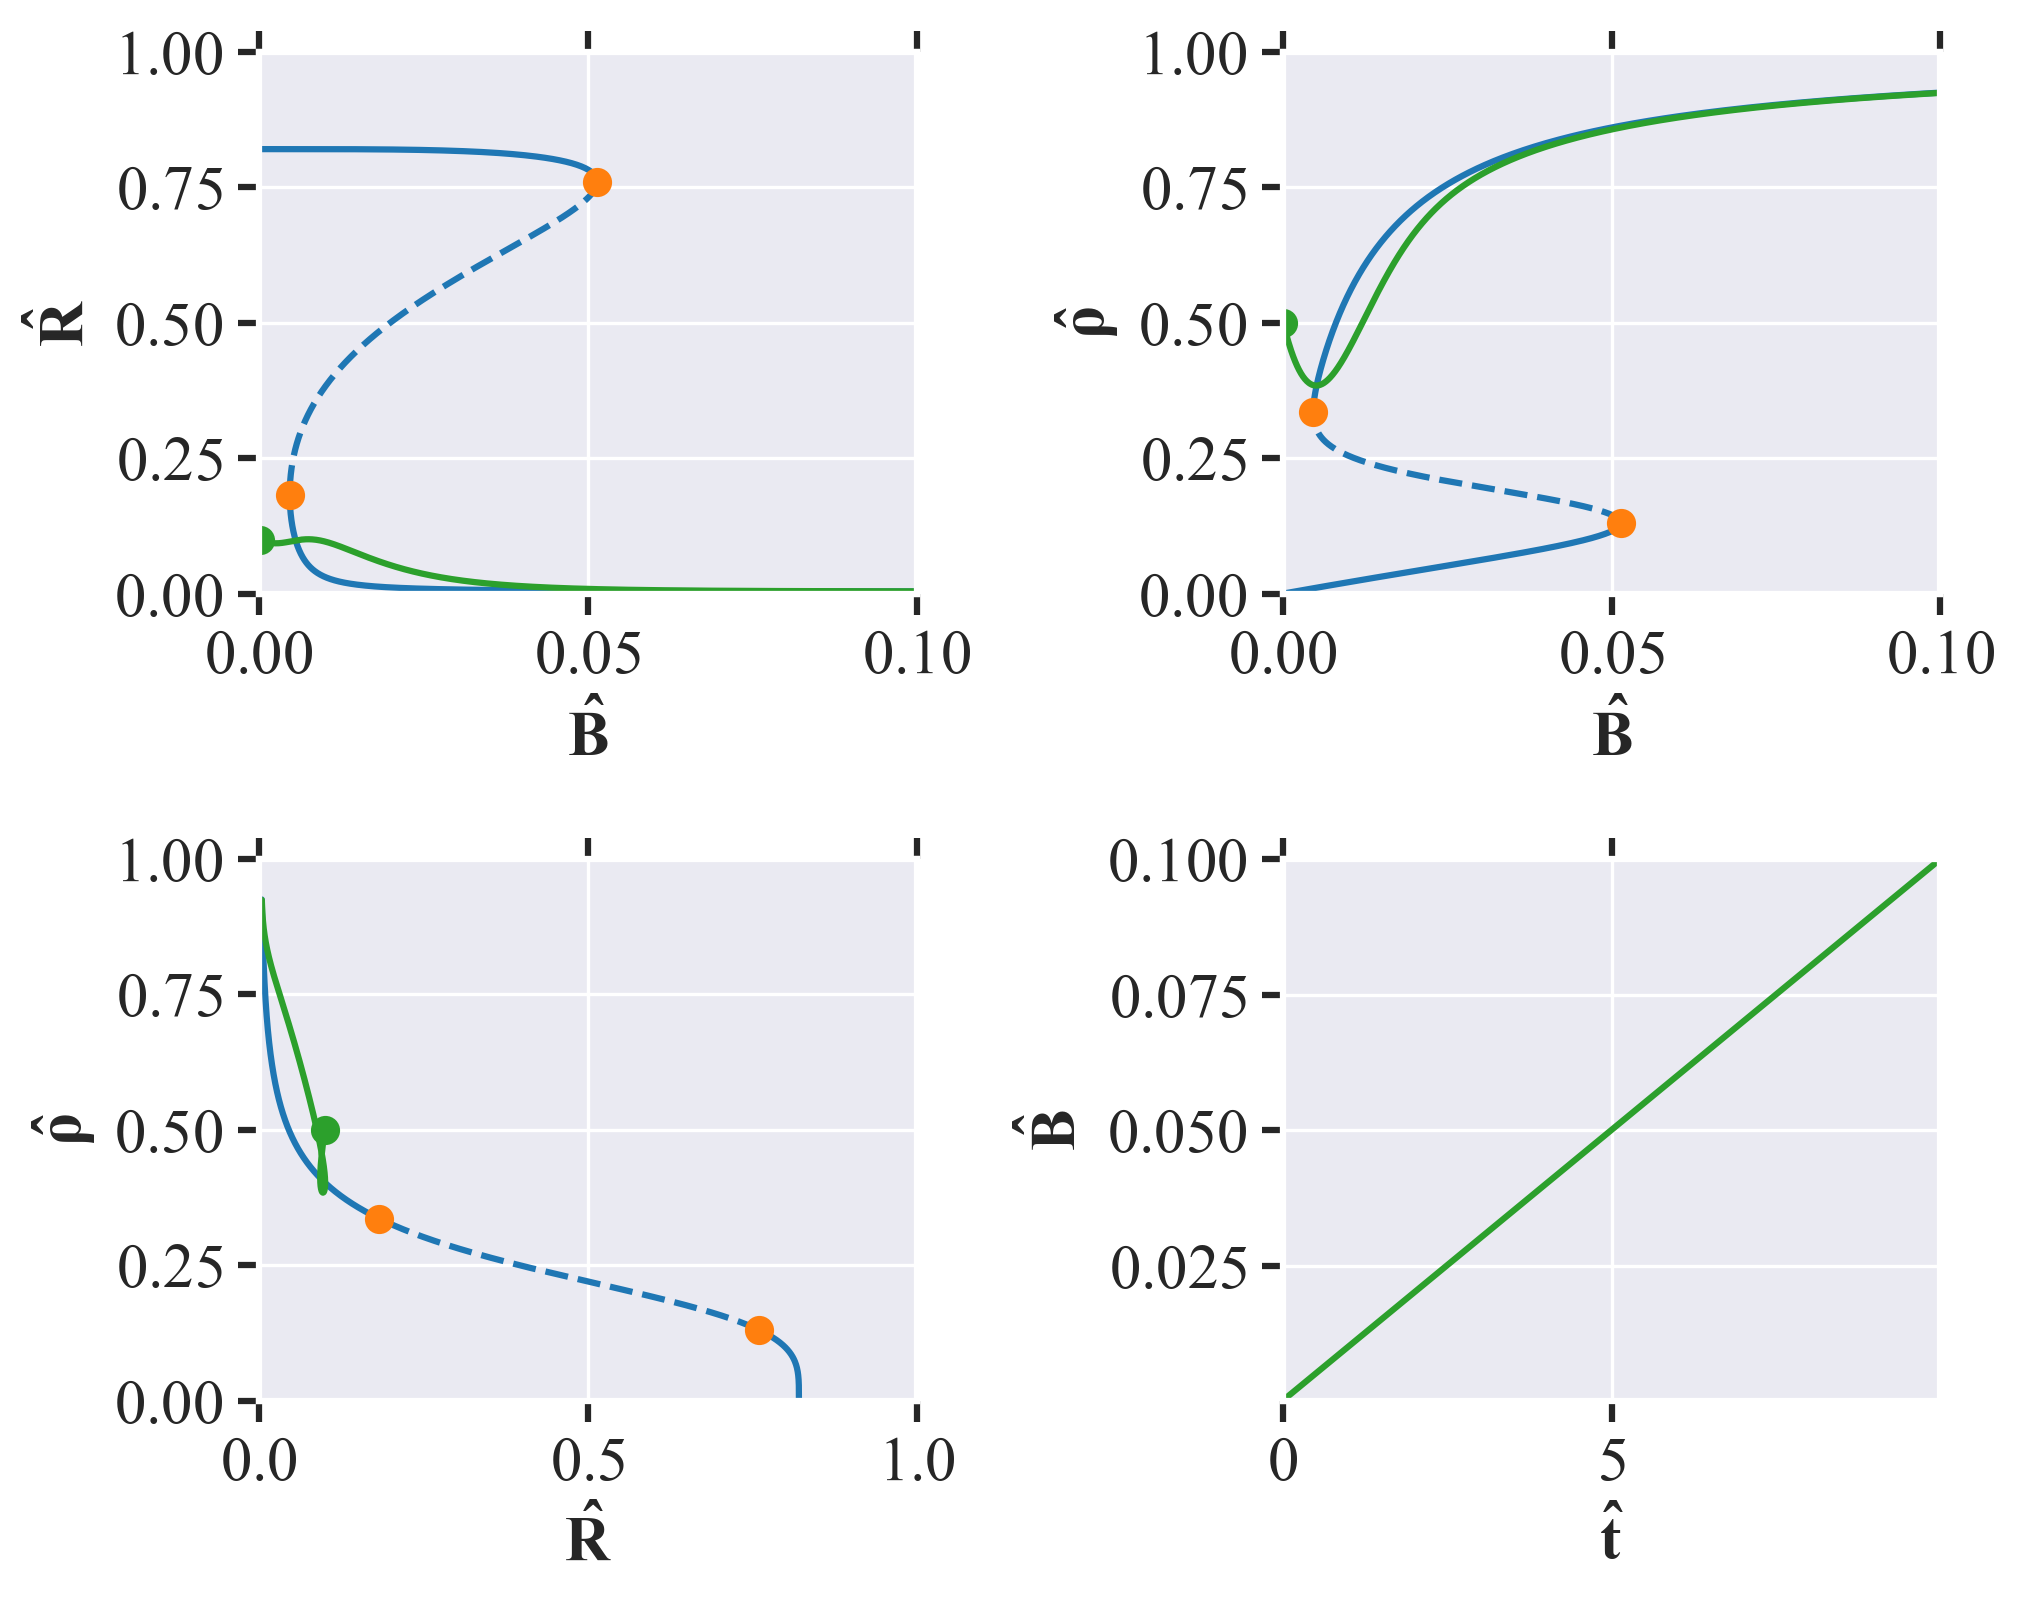
\includegraphics[width= \textwidth]{figures/cell_biology_R(0)=0.1_rho(0)=0.5_B(0)_0.0001_eps=0.01_Bmax=0.04.png}
    \caption{Equivalent to figure \ref{fig:cell_biology_ex3_small}, but now for big $\epsilon = 0.01$ and time horizon $T = 10$.}
    \label{fig:cell_biology_ex3_big}
\end{figure}

Next, we look for critical slowing down near the bifurcations of the system. The results for $\epsilon = 0.001$ and $\epsilon = 0.01$ are shown in figures \ref{fig:cell_biology_critical_slowing_down_small} and \ref{fig:cell_biology_critical_slowing_down_big} respectively.
\begin{figure}[H]
    \centering
    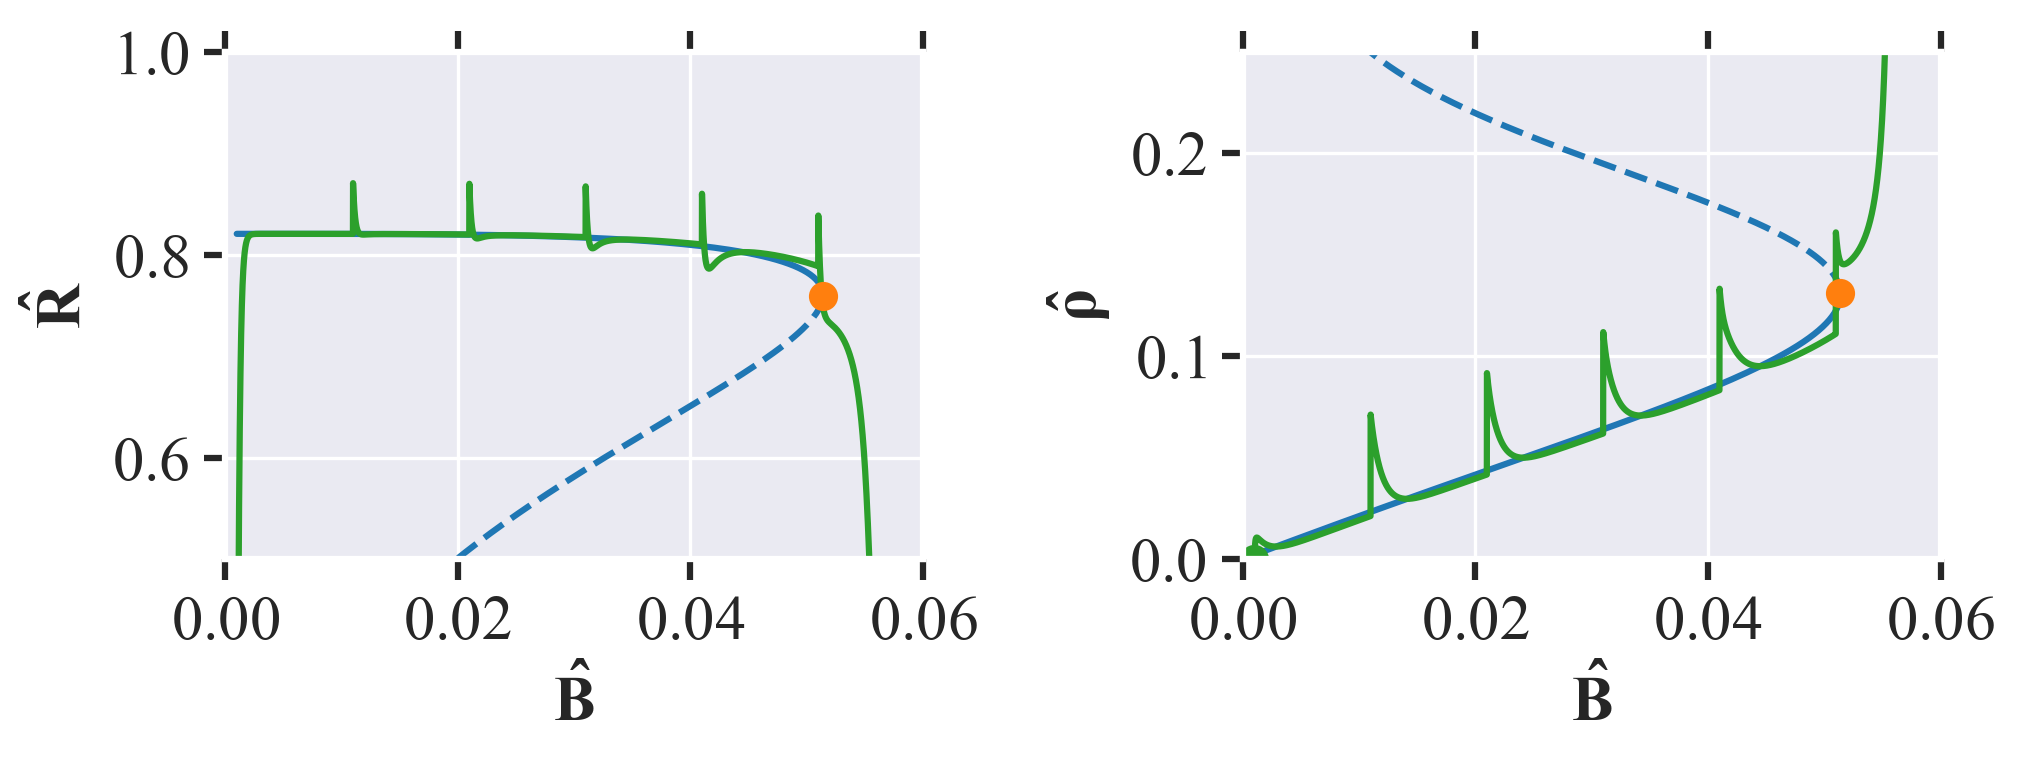
\includegraphics[width= \textwidth]{figures/cb_critslow_R(0)=0.0_rho(0)=0.0_B(0)_0.001_eps=0.001_Bmax=0.04.png}
    \caption{System behavior as it nears a turning point and under artificially added perturbations for $\epsilon = 0.001$. The perturbations are sufficiently 
    small and sparse in time to allow the system to restore to its equilibrium.}
    \label{fig:cell_biology_critical_slowing_down_small}
\end{figure}

\begin{figure}[H]
    \centering
    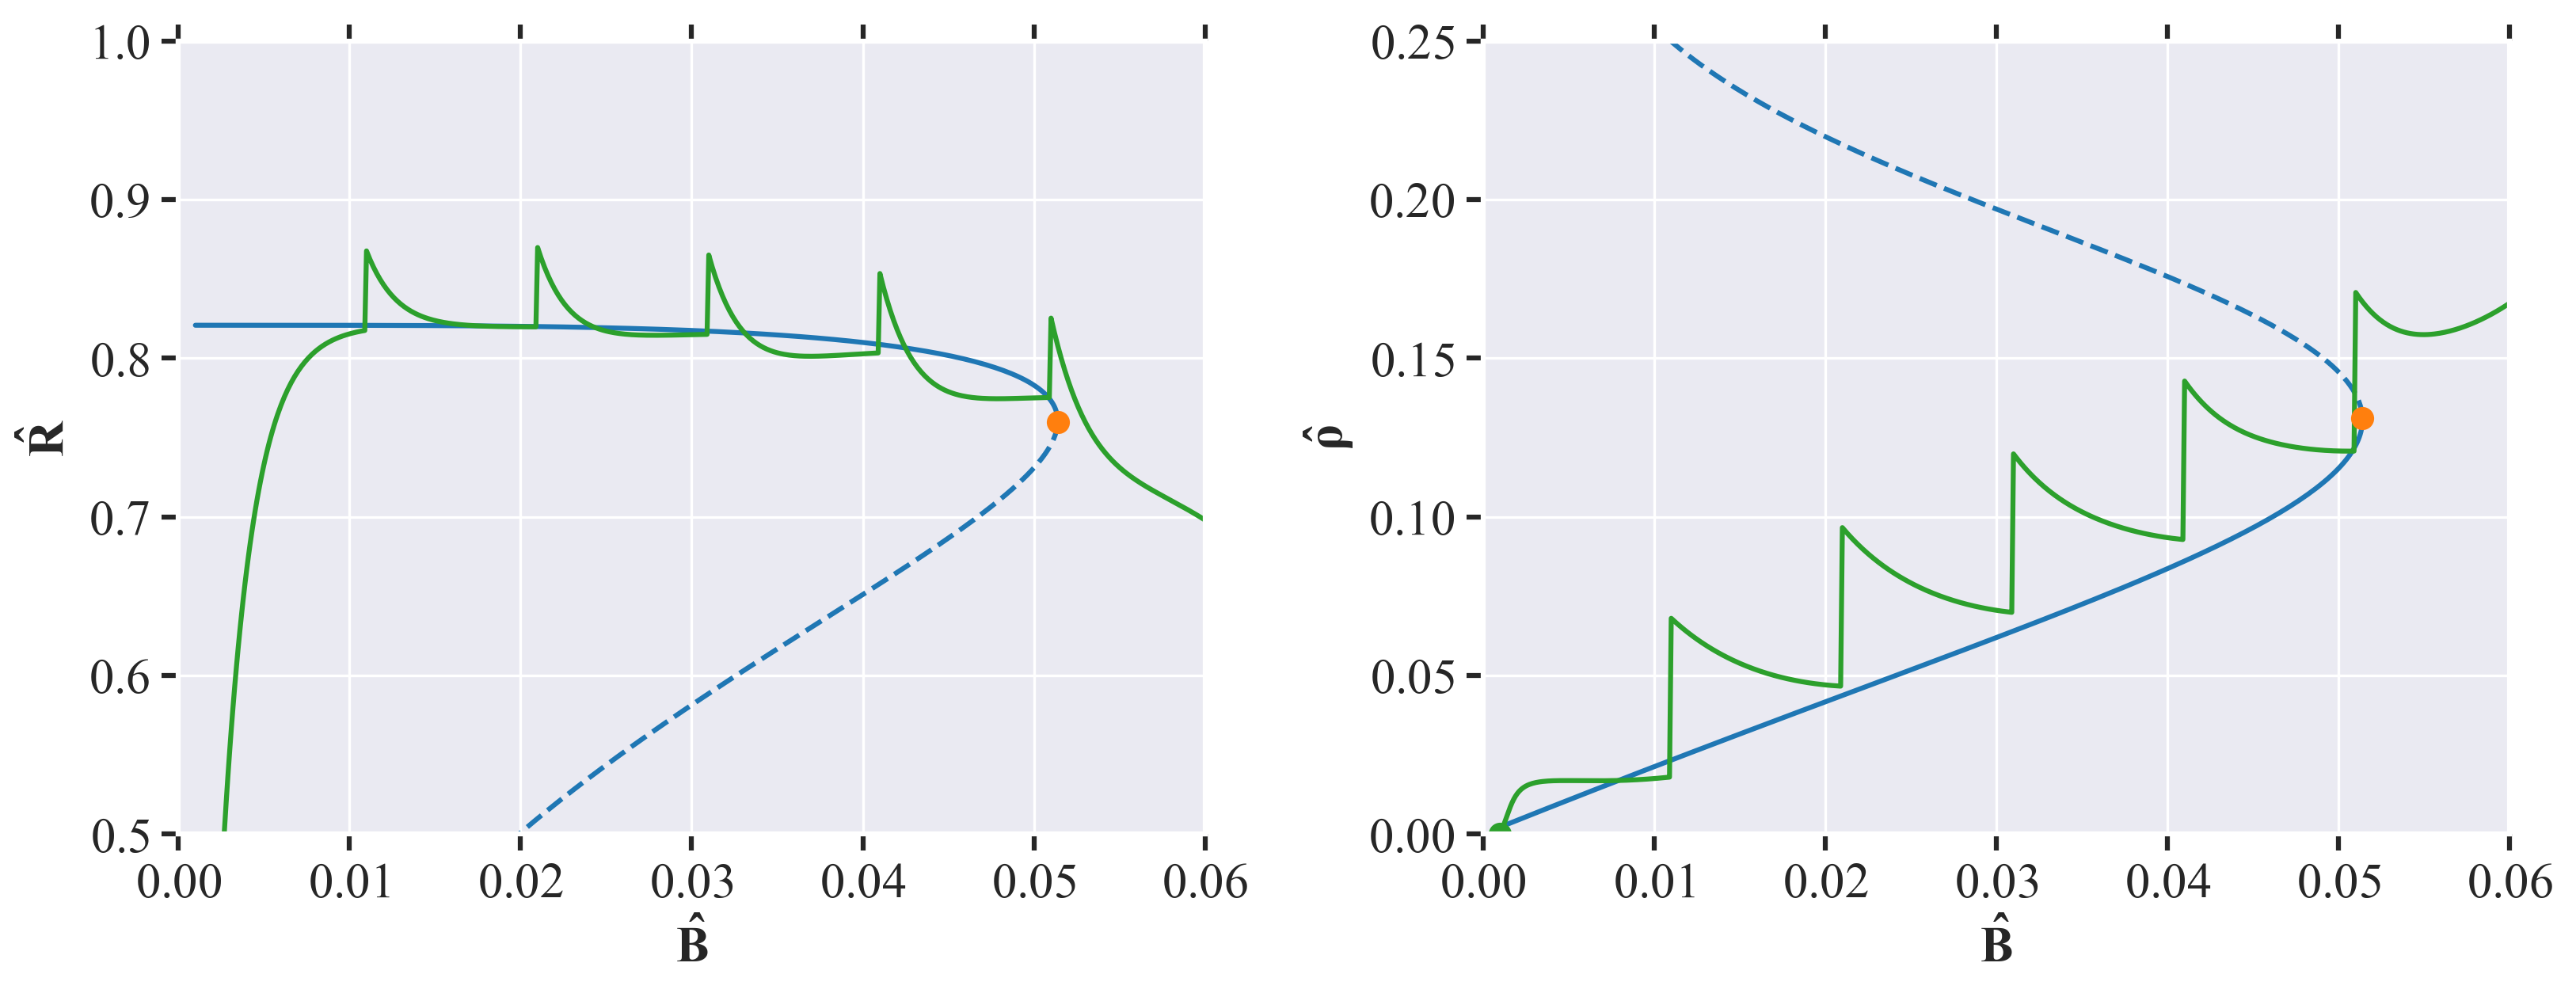
\includegraphics[width= \textwidth]{figures/cb_critslow_R(0)=0.0_rho(0)=0.0_B(0)_0.001_eps=0.01_Bmax=0.04.png}
    \caption{Exactly the same as figure \ref{fig:cell_biology_critical_slowing_down_small}, but now for $\epsilon = 0.01$. The perturbations are also the same,
    but are now too large and too frequent for the system to fully restore to its equilibrium.}
    \label{fig:cell_biology_critical_slowing_down_big}
\end{figure}

In both Figures \ref{fig:cell_biology_critical_slowing_down_small} and \ref{fig:cell_biology_critical_slowing_down_big}, we see that the system slows down in its convergence to the equilibrium near the turning point.
As a consequence, the system is  more sensitive to perturbations near the turning point. This is a clear example of critical slowing down. We also see that the system is more sensitive to perturbations when $\epsilon$ is larger.
This is because the system has less time to restore to its equilibrium before the next perturbation is applied. In other words, the critical slowing down is more pronounced when $\epsilon$ is larger. Additionally,
the final perturbation just before the turning point in all cases even causes the system to diverge from the equilibrium. This is because the system is already close to the turning point and the perturbation is too 
large to allow the system to restore to its equilibrium. Lastly, $\hat{R}_a$ seems to be more affected by this critical slowing down than $\hat{\rho}_a$.

The findings in this section are in line with the theory on critical slowing down. Indeed, as a system nears a bifurcation point, the eigenvalues of the corresponding linearized system approach zero. The restoration time of the system
is related to the reciprocal of these eigenvalues. As a result, the system slows down near the bifurcation point. This is exactly what we observe in the figures above.

\subsection{R-tipping}
We now introduce a super-linear time-dependent perturbation to $\hat{B}$. That is, the perturbed system is now given by
\begin{equation}
    \begin{cases}
        \hat{R}'_a &= \frac{\hat{A} \left(1 - \hat{R}_{a}\right)}{\hat{\rho}_a^{n} + \rho_{0}^{n}}  - \hat{\delta}_{R} \hat{R}_{a}\\
        \hat{\rho}'_a &= \frac{\hat{B} \left(1 - \hat{\rho}_a\right)}{\hat{R}_0^{n} + \hat{R}_{a}^{n}} - \hat{\rho}_a\\
        \hat{B}' &= \epsilon \frac{\hat{B}_{\textrm{max}}-\hat{B}}{\hat{B}_{\textrm{max}}},
    \end{cases}
\label{eq:cell_biology_R_tipping}
\end{equation}
Figures \ref{fig:cell_biology_R_tipping_small} and \ref{fig:cell_biology_R_tipping_big} show the continuation of the unperturbed system \ref{eq:cell_biology_R_tipping}, as well as a trajectory of  
system \ref{eq:cell_biology_R_tipping} for $\epsilon = 0.01$ and $\epsilon = 0.1$ respectively.

\begin{figure}[H]
    \centering
    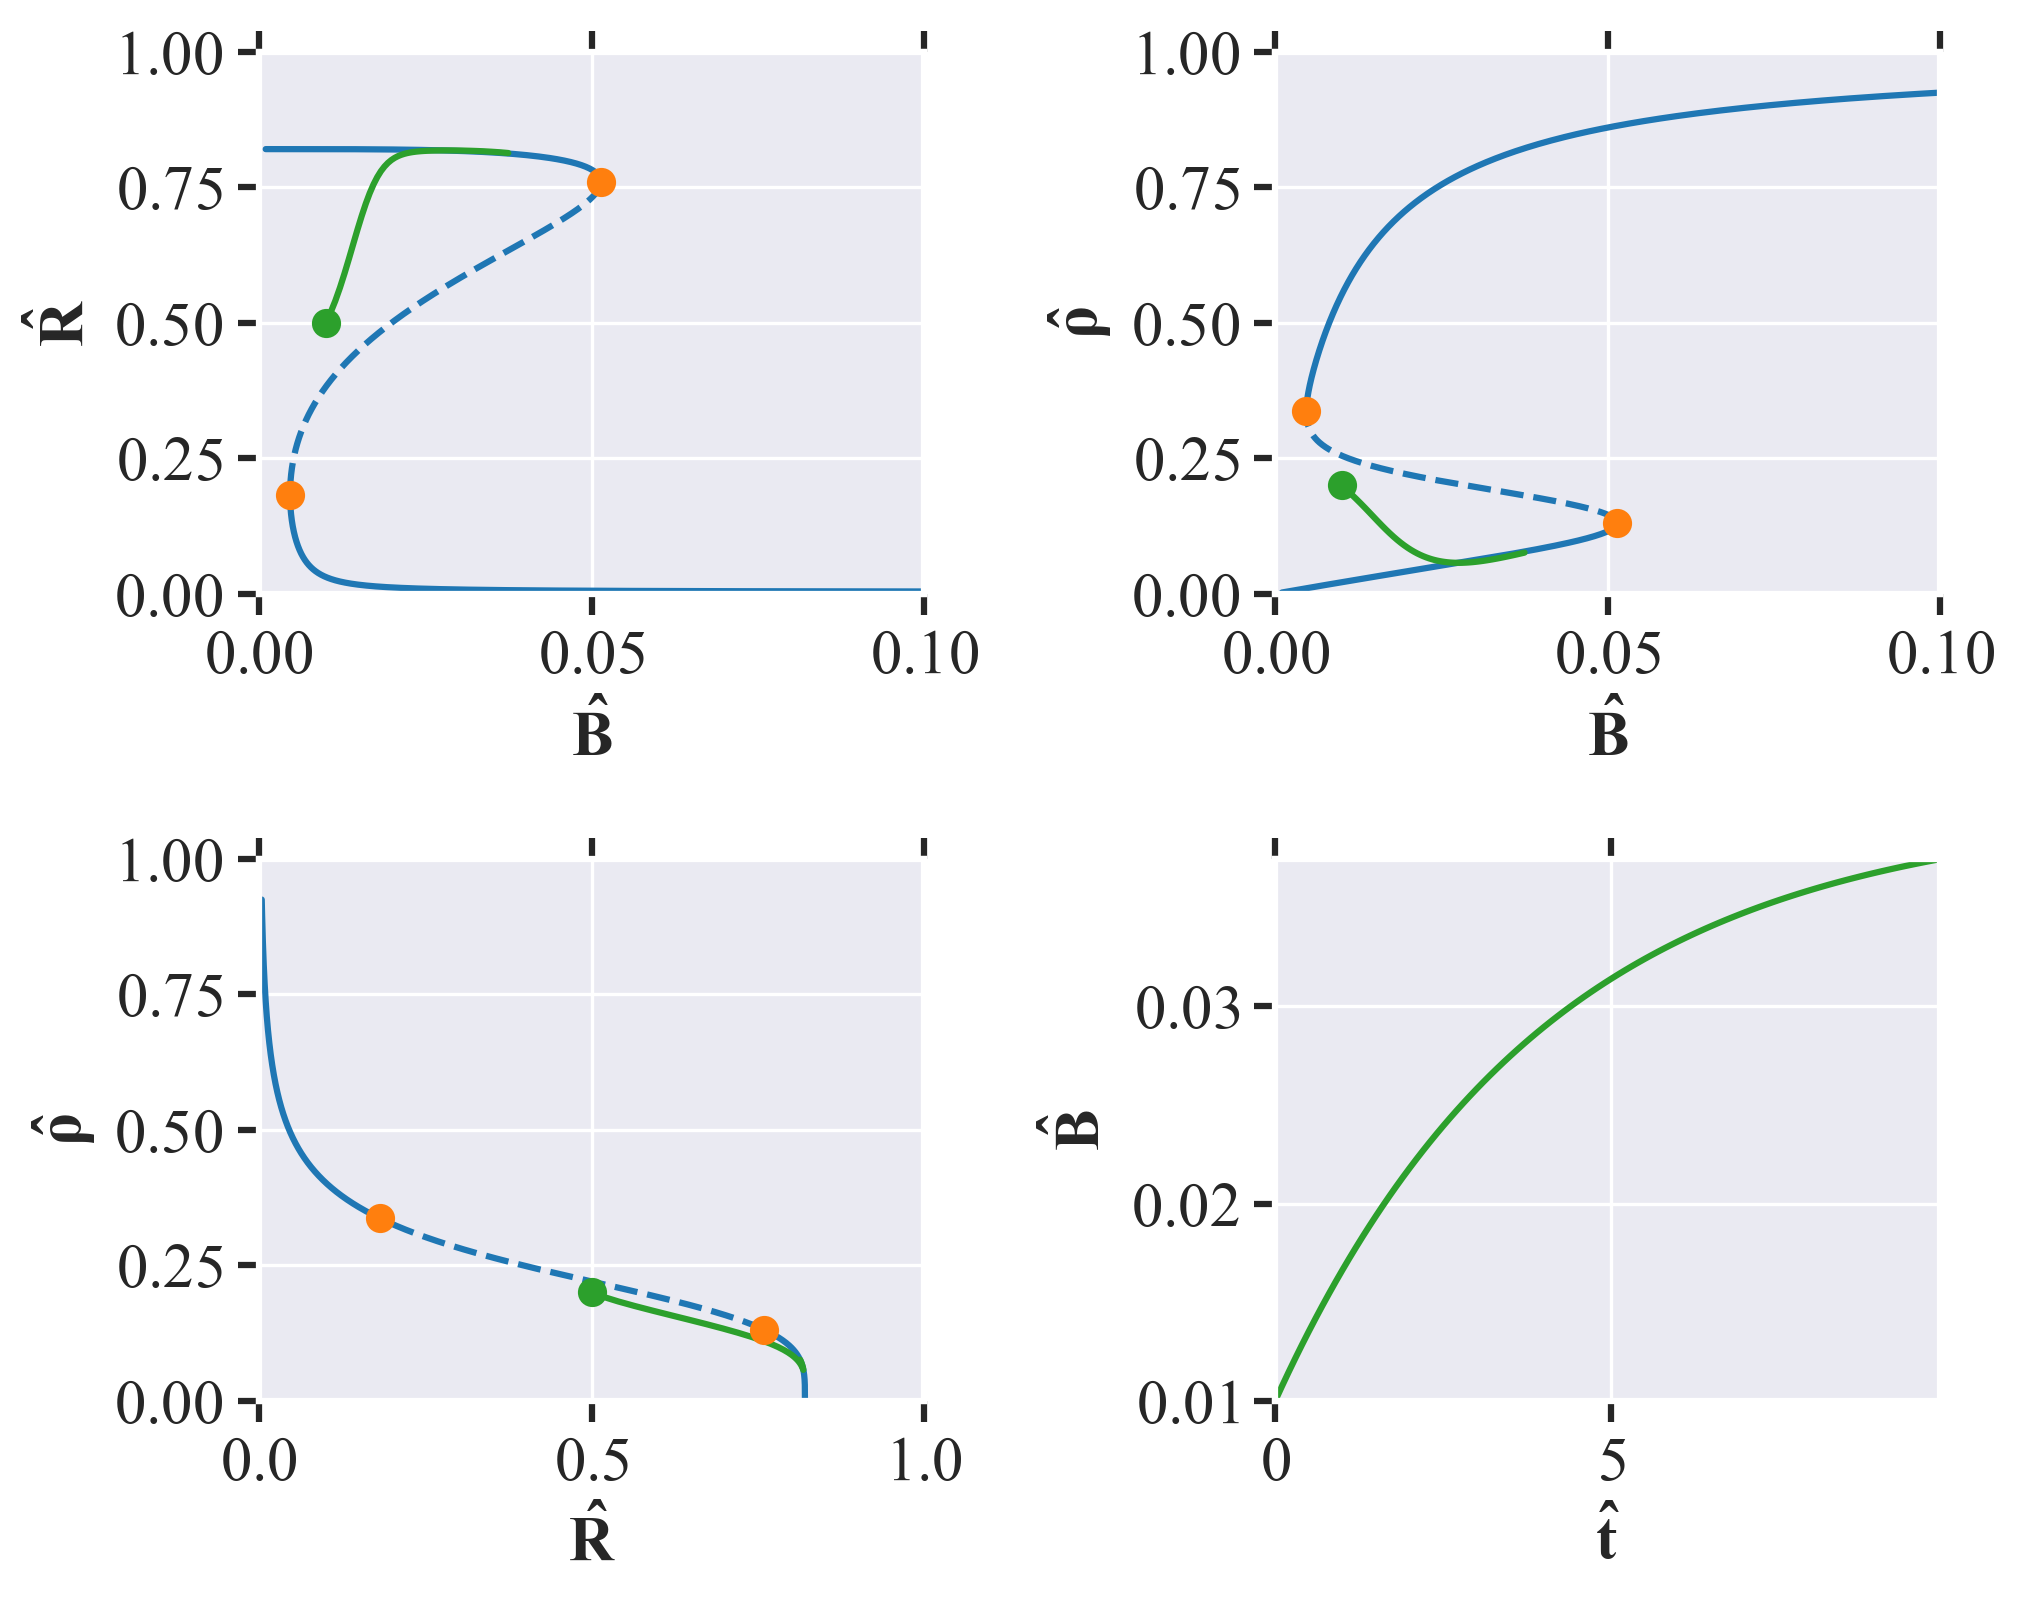
\includegraphics[width= \textwidth]{figures/cb_rtip_R(0)=0.5_rho(0)=0.2_B(0)_0.01_eps=0.01_Bmax=0.04.png}
    \caption{In this figure, we see the continuation of the unperturbed system \ref{eq:cell_biology_R_tipping} and a trajectory of the corresponding perturbed system for $\epsilon = 0.01$.
    The rate of the perturbation is small enough for the system to track the nearest equilibrium branch.}
    \label{fig:cell_biology_R_tipping_small}
\end{figure}

\begin{figure}[H]
    \centering
    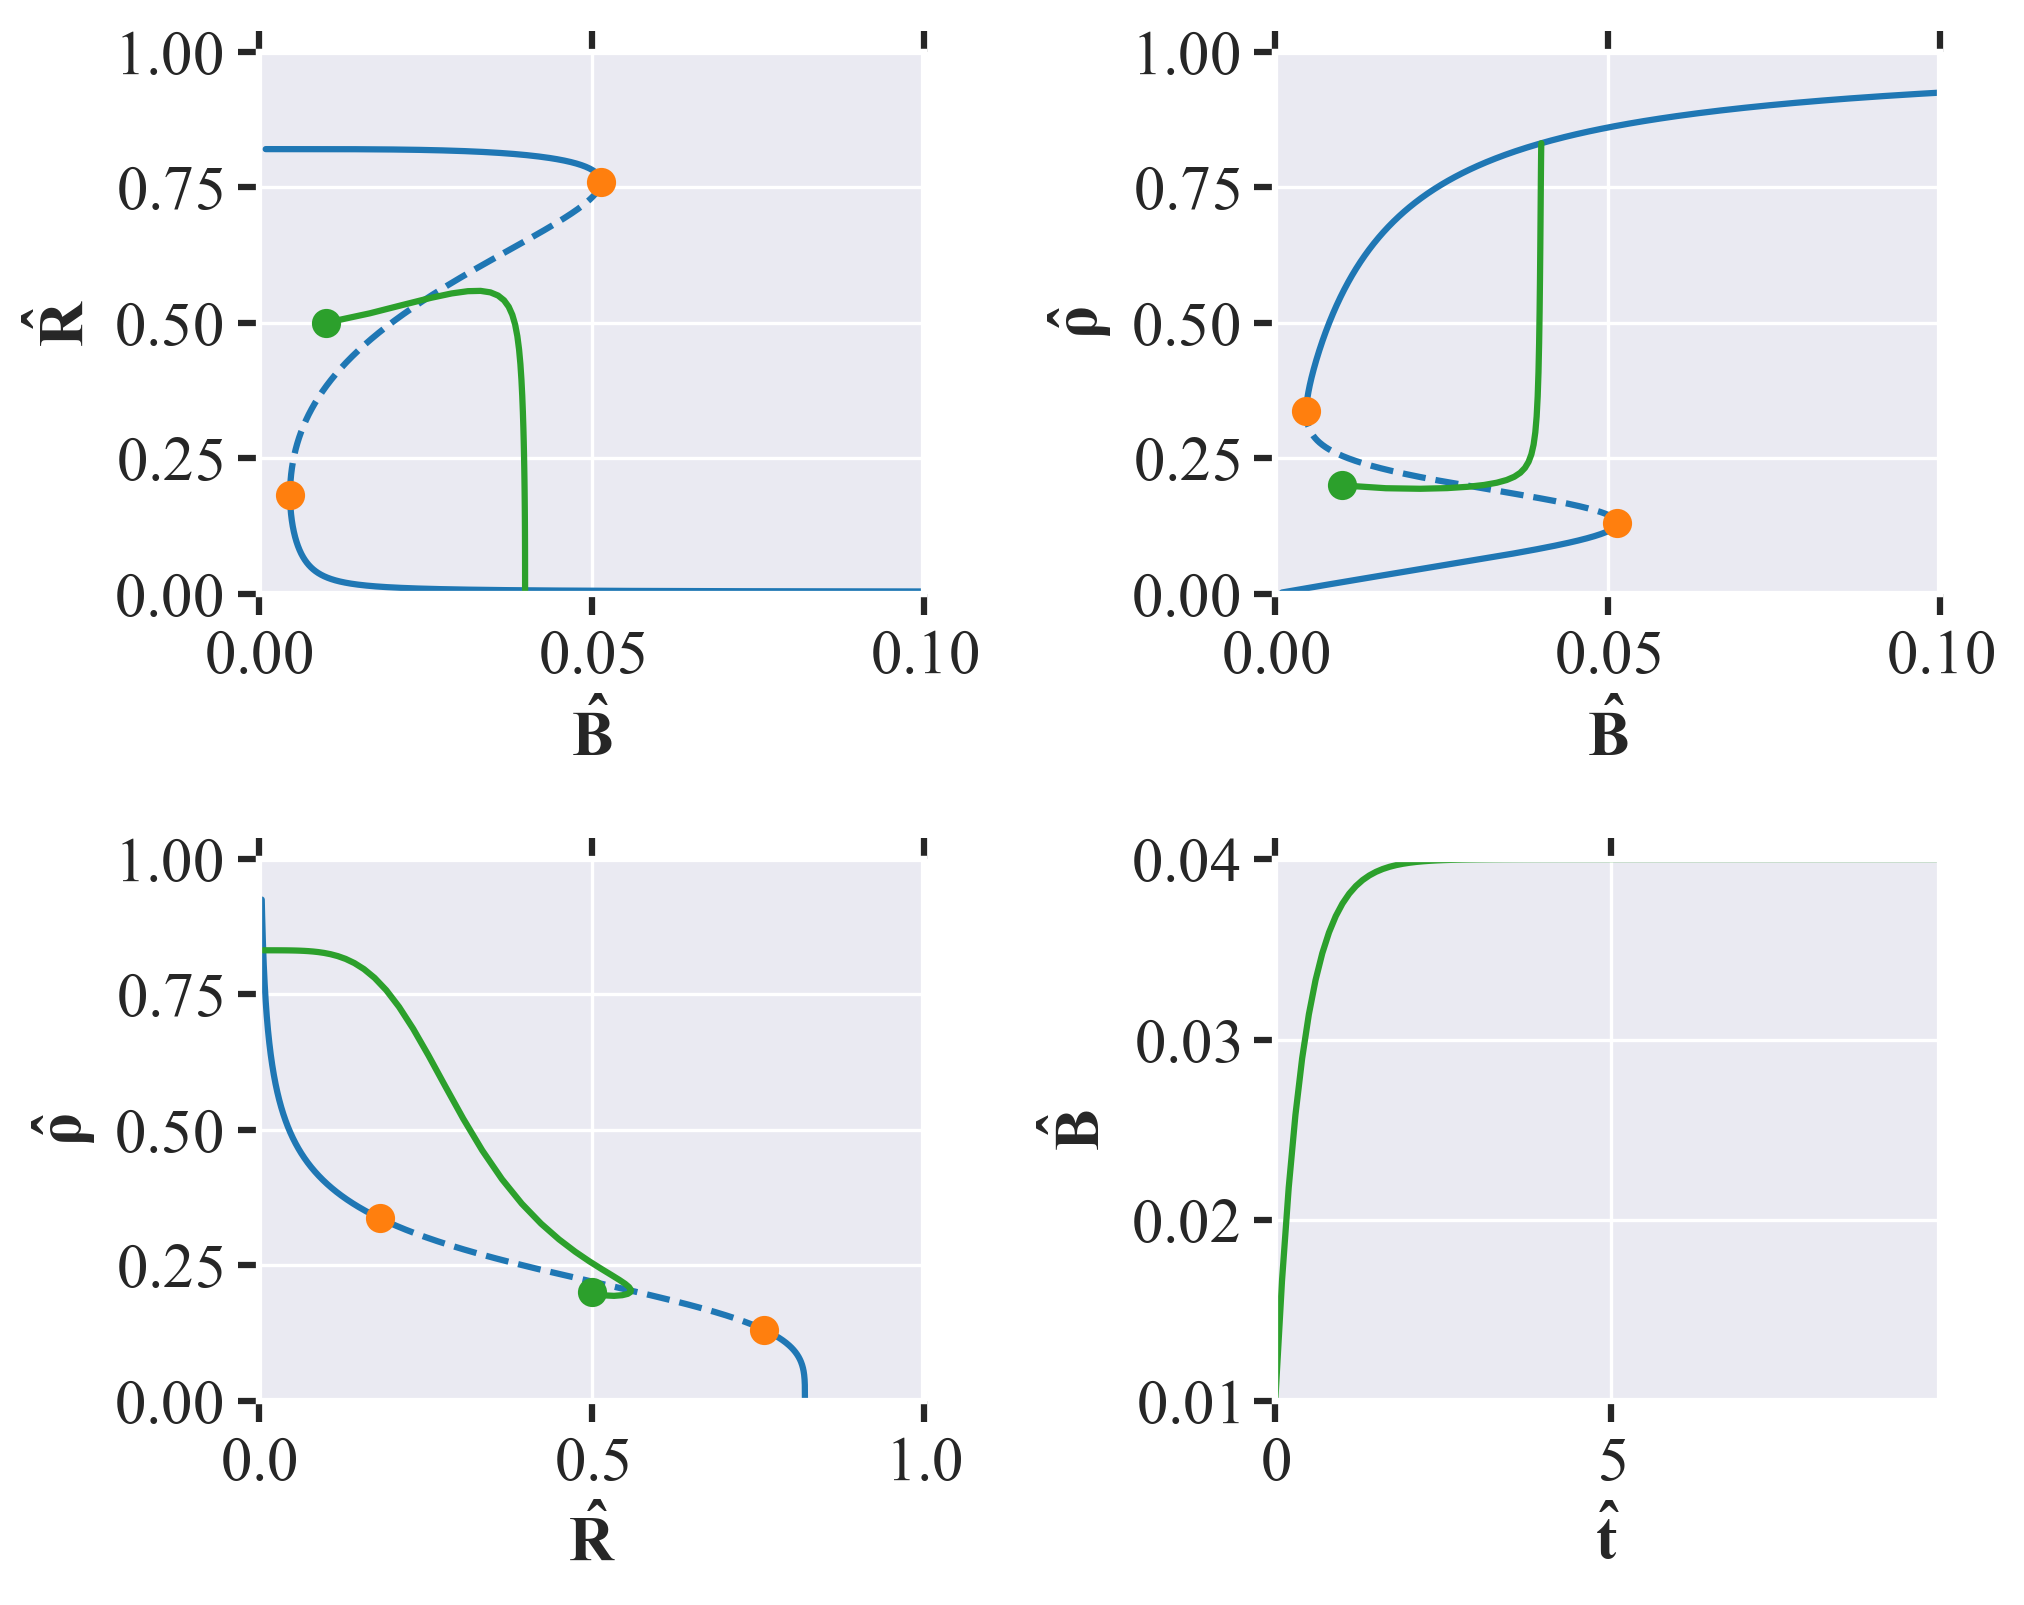
\includegraphics[width= \textwidth]{figures/cb_rtip_R(0)=0.5_rho(0)=0.2_B(0)_0.01_eps=0.1_Bmax=0.04.png}
    \caption{Equivalent to figure \ref{fig:cell_biology_R_tipping_small}, but now for $\epsilon = 0.1$. The rate of the perturbation is now too large for the system to track the nearest equilibrium branch.
    Instead, the system now jumps to the other equilibrium branch. This is a clear example of R-tipping.}
    \label{fig:cell_biology_R_tipping_big}
\end{figure}

\subsection{Conclusion}
In this assignment, we have studied the behavior of a system of ordinary differential equations that models the dynamics of a cell. 
We have seen that the system has two turning points, and that the system converges to one of the equilibrium points.
We have also seen a case of critical slowing down. This is a situation in which the system is more sensitive to artificially added perturbations near a bifurcation point, if $\epsilon$ (the rate of the parameter increase) is large 
compared to system dynamics (reciprocal of the linearized system's eigenvalues). These perturbations can cause the system to diverge from the equilibrium.
Lastly, we have observed R-tipping, in which a system can jump to another equilibrium branch for $\epsilon \approx 0.1$ and larger. 